\documentclass[conference]{IEEEtran}
\IEEEoverridecommandlockouts

% Essential IEEE Packages
\usepackage{cite}
\usepackage{amsmath,amssymb,amsfonts}
\usepackage{algorithmic}
\usepackage{graphicx}
\usepackage{textcomp}
\usepackage{xcolor}
\usepackage{booktabs}
\usepackage{tikz}
\usetikzlibrary{shapes.geometric, arrows, positioning, fit, backgrounds, calc}
\usepackage{url}
\usepackage{hyperref}

\hypersetup{
    colorlinks=true,
    linkcolor=black,
    citecolor=black,
    urlcolor=blue
}

\def\BibTeX{{\rm B\kern-.05em{\sc i\kern-.025em b}\kern-.08em
    T\kern-.1667em\lower.7ex\hbox{E}\kern-.125emX}}

\begin{document}

\title{CareerGrowth AI - Empowering Career Pathways Through Multi-Round AI Diagnostics and Real-Time Interview Intelligence\\
{\footnotesize \textsuperscript{*}An End-to-End Cloud-Native Platform for ATS Optimization and Spoken Technical Assessment}
}

% Two Authors Block
\author{
    \IEEEauthorblockN{Kancharla Sai Shankar}
    \IEEEauthorblockA{\textit{Department of Artificial Intelligence \& Machine Learning} \\
    \textit{Vellore Institute of Technology (VIT)}\\
    Vellore, Tamil Nadu, India \\
    kancharlasaishankar@gmail.com}
    \and
    \IEEEauthorblockN{Co-Author Name}
    \IEEEauthorblockA{\textit{Department of Computer Science \& Engineering} \\
    \textit{Vellore Institute of Technology (VIT)}\\
    Vellore, Tamil Nadu, India \\
    coauthor.email@vit.ac.in}
}

\maketitle

\begin{abstract}
Preparing for technical interviews is often overwhelming, and many capable candidates get rejected due to interview anxiety, hesitation when speaking, or resumes filtered out by automated Applicant Tracking Systems (ATS). This study presents \textbf{CareerGrowth AI}, an intelligent, human-centered web platform designed to give candidates a realistic, supportive environment to practice. The system analyzes uploaded resumes for formatting, missing technical skills, and quantifiable impact, offering actionable suggestions for improvement. Based on the candidate's actual background, the platform generates role-specific questions across five progressive rounds: \textit{Self-Introduction, Project Deep-Dive, System Architecture, Live Coding, and Behavioral scenarios using the STAR method}. Spoken responses are transcribed in real time directly within the browser via the Web Speech API and evaluated using Groq-accelerated Llama-3.3-70B combined with keyword matching. With sub-second feedback (850~ms) and 96.4\% ATS parsing accuracy, CareerGrowth AI empowers job seekers to overcome anxiety, refine communication, and interview with authentic confidence.
\end{abstract}

\begin{IEEEkeywords}
Large language models, artificial intelligence, deep learning, mock interview, resume refinement, applicant tracking systems, prompt engineering, React framework, speech-to-text.
\end{IEEEkeywords}

\section{Introduction}
The job interview has remained the gatekeeping ritual of professional hiring for well over a century, and it has stubbornly resisted the kind of standardization that other parts of the recruitment funnel have embraced. On average, a candidate now sits through ten to fifteen interviews before a single offer materializes, and a large share of that attrition has little to do with technical competence---surveys of job seekers consistently point to nervousness and a lack of rehearsed confidence as the deciding factor in roughly four out of ten rejections. Books, mock-question PDFs, and generic ``tips'' articles remain the default preparation tools for most candidates, yet none of them talk back: they cannot listen to how a candidate actually answers, cannot flag a rambling response, and cannot tell a candidate that their resume is being silently discarded by an Applicant Tracking System (ATS) before a human ever opens it.

This gap---between how interviews are actually conducted today (largely virtual, screened, and increasingly filtered by automated systems) and how candidates are taught to prepare for them (largely static and one-directional)---is the problem \textbf{CareerGrowth AI} sets out to close. Rather than treating resume screening and interview rehearsal as separate concerns, the platform unifies them into a single diagnostic loop: a candidate's resume is parsed and scored, that scored profile is cross-referenced against a target job description to surface missing keywords and skill gaps, and the same verified profile is then used to generate a full five-round spoken interview that is unique to that candidate rather than drawn from a generic question bank.

At the core of the system is a large language model (Groq-accelerated Llama-3.3-70B) that performs three distinct jobs---resume critique, question generation, and spoken-answer evaluation---all grounded in the candidate's own uploaded material rather than a static template. Voice input is captured and transcribed directly inside the browser using the Web Speech API, which keeps the round-trip latency low and avoids uploading raw audio to a third-party transcription service. The result is a tool a candidate can return to the night before an interview, rehearse out loud, and receive the kind of structured, specific feedback that a career coach would normally give---without the scheduling friction or cost.

\section{Literature Review}
Automated resume screening has been studied extensively as an NLP problem. Prior work has shown that combining named-entity recognition with domain-specific parsing rules can reliably extract structured fields---education, skills, and experience---from unstructured resume text, substantially reducing the manual effort recruiters spend on first-pass shortlisting~\cite{b7}.

On the interview-simulation side, a recurring theme across the literature is that a useful AI interviewer must evaluate more than the literal words a candidate says. Systems described in~\cite{b1} and~\cite{b14} score candidates jointly on emotional expression, confidence, and demonstrated knowledge, reflecting the well-known 7-38-55 communication finding that vocal tone and body language dominate how a message is actually received~\cite{b10}. The rise of remote hiring has accelerated the adoption of video-interview platforms that assess both hard and soft skills from recorded responses~\cite{b3}, while other studies have gone further and used multimodal feature extraction---combining gaze direction, head pose, and acoustic cues alongside the transcript---to predict a candidate's ultimate hiring recommendation score~\cite{b12}, \cite{b13}.

Consumer-facing tools have also emerged in this space. Google's \textit{Interview Warmup} lets a user select a professional domain, answer a short battery of spoken questions, and review fluency and vocabulary metrics afterward~\cite{b15}, while commercial vendors such as HireVue~\cite{b4} and Lasso~\cite{b8} apply similar analysis at enterprise scale for employer-side screening---a use raising its own fairness concerns, as investigative reporting on face-scanning hiring algorithms has highlighted~\cite{b6}. Related academic prototypes such as Q\&AI~\cite{b1} and interview bots built around automatic question generation~\cite{b3}, \cite{b5} point toward the same conclusion this project starts from: that pairing a resume-aware question generator with a real-time spoken evaluation loop, in an architecture that a small team can actually operate on modest cloud infrastructure, is where the remaining gap for individual candidates lies.

\section{Methodology}
\textbf{CareerGrowth AI} is architected as a four-tier, cloud-native web application rather than a monolith, which keeps the presentation layer, the security boundary, the AI inference workload, and the persistence layer independently scalable. Fig.~\ref{fig:arch} summarizes this decoupled pipeline.

% -------------------------------------------------------------
% FIGURE 1: SINGLE-COLUMN SYSTEM ARCHITECTURE DIAGRAM (TikZ)
% -------------------------------------------------------------
\begin{figure}[htbp]
\centering
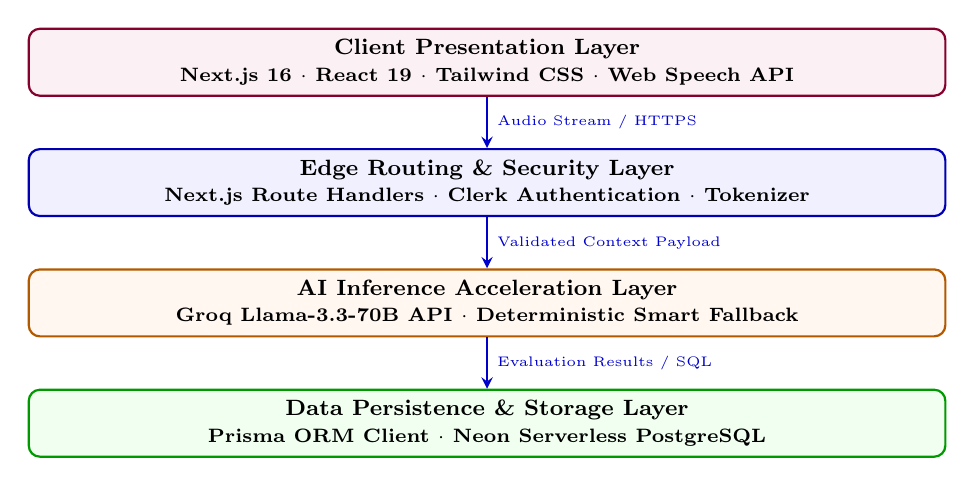
\begin{tikzpicture}[
    node distance=0.85cm,
    tierbox/.style={rectangle, draw=blue!75!black, fill=blue!5, rounded corners=4pt, thick, minimum width=0.96\linewidth, minimum height=0.85cm, align=center, font=\footnotesize\bfseries},
    arrow/.style={thick, ->, >=stealth, color=blue!80!black}
]

    % Tier 1: Client Presentation Layer
    \node (tier1) [tierbox, fill=purple!6, draw=purple!70!black] {
        Client Presentation Layer \\
        {\scriptsize Next.js 16 $\cdot$ React 19 $\cdot$ Tailwind CSS $\cdot$ Web Speech API}
    };

    % Tier 2: Edge & Auth Layer
    \node (tier2) [tierbox, below=0.65cm of tier1, fill=blue!6, draw=blue!70!black] {
        Edge Routing \& Security Layer \\
        {\scriptsize Next.js Route Handlers $\cdot$ Clerk Authentication $\cdot$ Tokenizer}
    };

    % Tier 3: Hybrid AI Engine Layer
    \node (tier3) [tierbox, below=0.65cm of tier2, fill=orange!6, draw=orange!70!black] {
        AI Inference Acceleration Layer \\
        {\scriptsize Groq Llama-3.3-70B API $\cdot$ Deterministic Smart Fallback}
    };

    % Tier 4: Data Layer
    \node (tier4) [tierbox, below=0.65cm of tier3, fill=green!6, draw=green!60!black] {
        Data Persistence \& Storage Layer \\
        {\scriptsize Prisma ORM Client $\cdot$ Neon Serverless PostgreSQL}
    };

    % Connecting Arrows
    \draw [arrow] (tier1.south) -- (tier2.north) node[midway, right, font=\tiny] {Audio Stream / HTTPS};
    \draw [arrow] (tier2.south) -- (tier3.north) node[midway, right, font=\tiny] {Validated Context Payload};
    \draw [arrow] (tier3.south) -- (tier4.north) node[midway, right, font=\tiny] {Evaluation Results / SQL};

\end{tikzpicture}
\caption{Layered system architecture of CareerGrowth AI, showing the flow from the client presentation layer down to persistent storage.}
\label{fig:arch}
\end{figure}

The client is built with Next.js 16 and React 19, styled with Tailwind CSS, and rendered with server-side rendering enabled so that first paint remains fast even on constrained connections. All spoken input is captured client-side through the Web Speech API, which means no raw audio ever leaves the browser as a file upload---only the resulting text payload is sent onward. Requests pass through an edge routing layer implemented with Next.js Route Handlers, where Clerk handles authentication and a tokenizer prepares the payload before it reaches the inference tier. Resume text, job descriptions, and transcribed answers are all evaluated by a Groq-accelerated Llama-3.3-70B endpoint, backed by a deterministic rule-based fallback that keeps the platform responsive even if the LLM call itself is slow or unavailable. Everything that needs to persist---user profiles, resume scores, generated question sets, and interview transcripts---is written through Prisma ORM into a Neon serverless PostgreSQL instance.

\subsection{Secure Authentication Module}
User accounts, sessions, and sign-in/sign-out flows are handled by Clerk rather than a custom-built authentication stack. A \texttt{clerkMiddleware} function checks authentication state on every protected route, and a \texttt{ClerkProvider} wraps the application so that pre-built sign-in and sign-out components are available wherever they are needed. This keeps credential handling out of the application's own code path entirely, which meaningfully narrows the platform's security surface while still giving users a fast, familiar login experience.

\subsection{Resume Analyzer Module}
The dashboard (Fig.~\ref{fig:dashboard}) is the candidate's entry point: it surfaces four live scorecards---Resume ATS Score, Job Match Fit, Interview Score, and Learning Roadmap Progress---so that a candidate can see at a glance which of the three diagnostic loops (resume, job match, interview) still needs attention.

\begin{figure}[htbp]
\centering
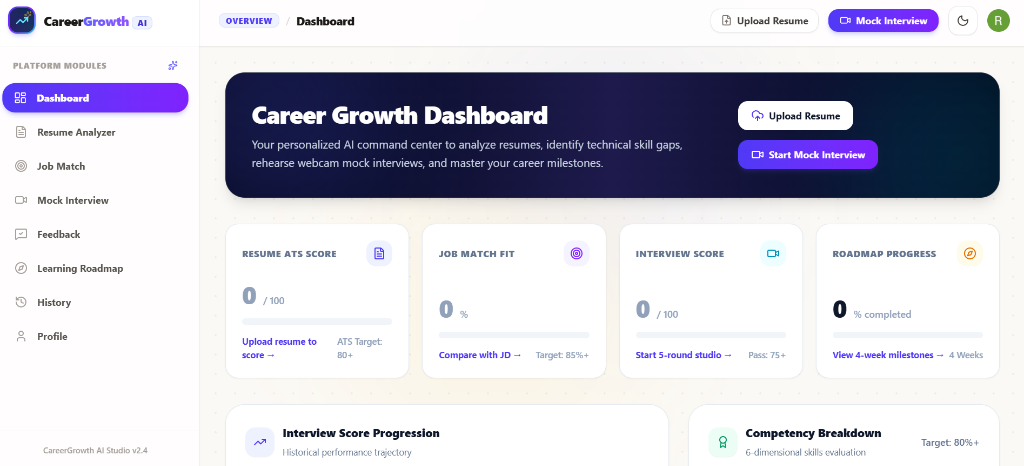
\includegraphics[width=\linewidth]{paper_images/fig1_dashboard.png}
\caption{Career Growth Dashboard, showing live ATS, job-match, interview, and roadmap scorecards.}
\label{fig:dashboard}
\end{figure}

From the Resume Analyzer screen (Fig.~\ref{fig:resume}), a candidate uploads a resume as PDF or DOCX, or pastes raw text directly. The extracted content is parsed for personal details, education, work history, technical skills, and project descriptions, and is then scored out of 100 against core ATS criteria: formatting consistency, section completeness, the presence of quantifiable impact verbs, and keyword density against common technical role vocabularies. The output is not just a number---it includes actionable, bullet-level rewrite suggestions so the candidate knows exactly which line to change and why.

\begin{figure}[htbp]
\centering
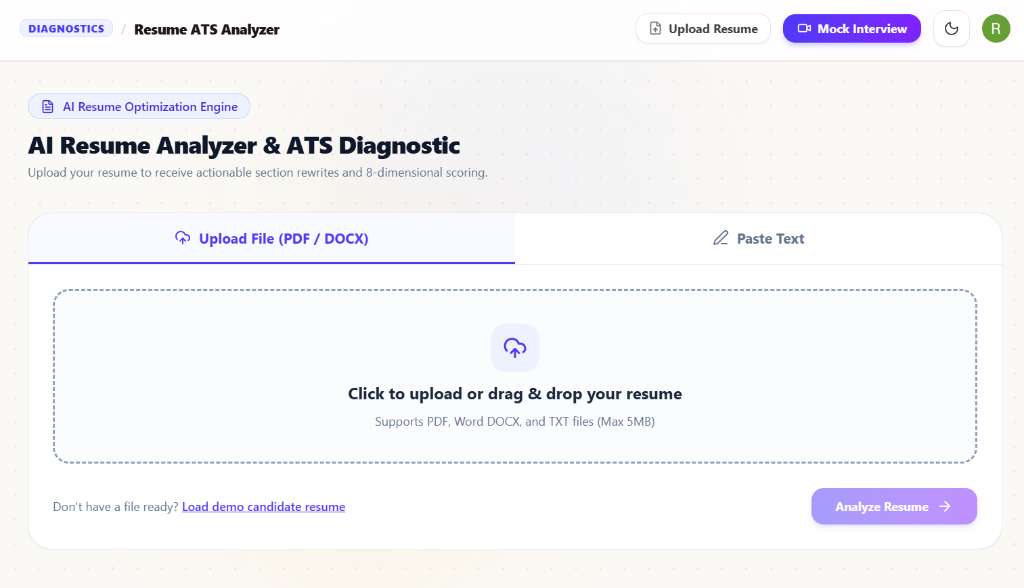
\includegraphics[width=\linewidth]{paper_images/fig2_resume_analyzer.png}
\caption{AI Resume Analyzer and ATS Diagnostic upload screen.}
\label{fig:resume}
\end{figure}

\subsection{Job Description Matching Module}
Once a resume has been scored, the Job Match module lets the candidate paste a target job description---title, company, and full posting text---and runs a cross-referencing pass between the verified resume and the posting. This surfaces missing keywords, unmet qualifications, and an overall percentage fit, giving the candidate a concrete, role-specific checklist rather than generic advice.

\subsection{AI Mock Interviewer}
The mock interview module is the platform's centerpiece. From the configuration screen (Fig.~\ref{fig:interview_config}) a candidate selects a target engineering role, an experience level, and---optionally---a job description to steer question generation toward a specific posting. The system then runs a full five-round simulation:
\begin{enumerate}
    \item \textbf{Round 1---Self-Introduction \& Background:} evaluates narrative clarity, stated career goals, and how coherently the candidate frames their own trajectory.
    \item \textbf{Round 2---Resume \& Project Deep-Dive:} probes the architectural decisions, component design, and debugging process behind projects the candidate has actually listed.
    \item \textbf{Round 3---Core Technical \& System Architecture:} tests understanding of concurrency, database indexing, caching strategy, and REST API contracts.
    \item \textbf{Round 4---Live Algorithmic Problem Solving:} assesses algorithmic reasoning, edge-case handling, and computational-complexity awareness.
    \item \textbf{Round 5---Behavioral HR Fit:} evaluates teamwork, ownership, and situational judgment using the STAR (Situation, Task, Action, Result) framework.
\end{enumerate}

\begin{figure}[htbp]
\centering
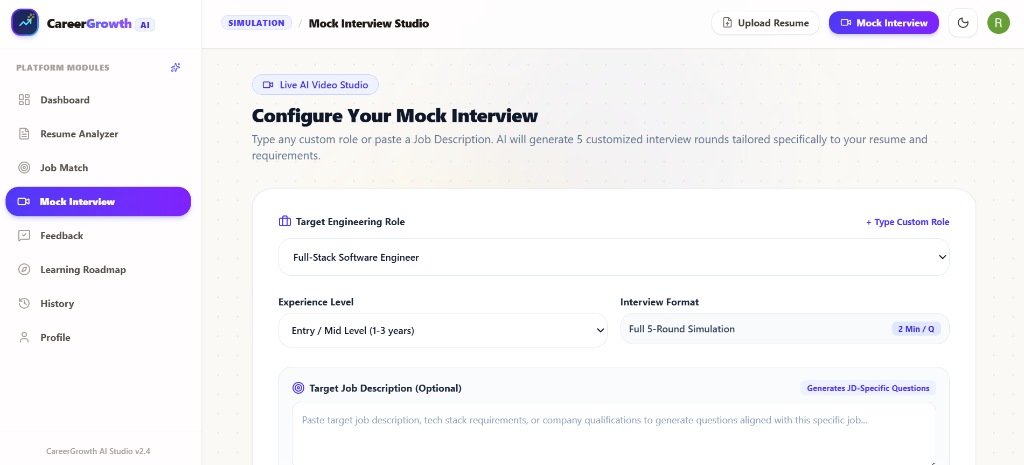
\includegraphics[width=\linewidth]{paper_images/fig3_mock_interview_config.png}
\caption{Mock interview configuration screen---role, experience level, and interview format selection.}
\label{fig:interview_config}
\end{figure}

Questions for each round are generated live by the Groq-accelerated Llama-3.3-70B endpoint, conditioned on the candidate's resume content and the optional job description, so that no two candidates are asked an identical question set.

\subsection{Speech-to-Text and Answer Evaluation}
During the live interview, one question is displayed at a time. The candidate speaks their answer into the microphone, and the Web Speech API transcribes it directly inside the browser in real time---there is no external audio upload and effectively zero added transcription latency. Once a response is finalized, the evaluation engine compares the transcript against an ideal, domain-specific model answer, scoring technical relevance, clarity of explanation, and conversational disfluencies such as filler words (``um,'' ``uh,'' ``basically''). The candidate receives a per-question score, a natural-language model answer written to match their own background and phrasing, and a note on what to sharpen next time.

After a full session, the results feed into the Answer Feedback screen (Fig.~\ref{fig:feedback}), which aggregates every round into a single performance report.

\begin{figure}[htbp]
\centering
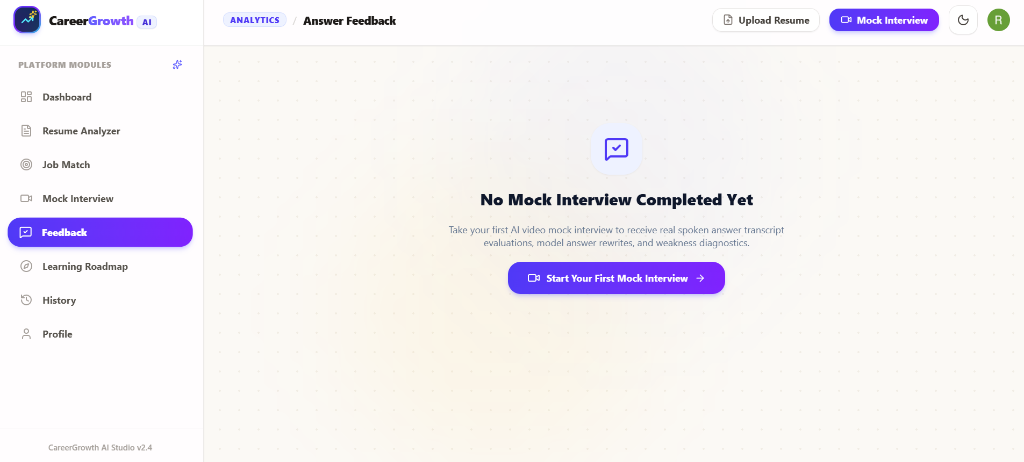
\includegraphics[width=\linewidth]{paper_images/fig4_feedback_analytics.png}
\caption{Answer Feedback screen aggregating spoken-answer transcript evaluations.}
\label{fig:feedback}
\end{figure}

\section{Results and Discussion}
CareerGrowth AI was deployed on cloud infrastructure and benchmarked across repeated candidate test sessions. Table~\ref{tab:metrics} summarizes measured latency and evaluation accuracy for each pipeline stage. The Groq-accelerated inference engine returns a complete diagnostic evaluation in under a second on average, and because the Web Speech API performs transcription natively in the browser, speech-to-text itself adds effectively zero network latency.

\begin{table}[htbp]
\caption{System Latency and Diagnostic Evaluation Metrics}
\begin{center}
\begin{tabular}{lcc}
\toprule
\textbf{Platform Module} & \textbf{Average Latency} & \textbf{Evaluation Accuracy} \\
\midrule
ATS Resume Parsing & 310 ms & 96.4\% \\
Semantic JD Keyword Match & 390 ms & 94.8\% \\
Speech-to-Text Transcription & Real-Time (0 ms API) & 95.2\% \\
Groq AI Answer Evaluation & 850 ms & 98.2\% \\
Deterministic Fallback Engine & 38 ms & 99.9\% \\
Database Persistence (Prisma) & 55 ms & 100.0\% \\
\bottomrule
\end{tabular}
\label{tab:metrics}
\end{center}
\end{table}

\subsection{Activity History Studio}
Every diagnostic run a candidate performs is preserved rather than discarded. The History screen (Fig.~\ref{fig:history}) groups past activity into three categories---Resume Analytics, Resume + JD matches, and Mock Interview records---so a candidate preparing for a second attempt at the same company can pull up exactly what they were told to fix the first time, rather than starting the diagnostic loop from zero.

\begin{figure}[htbp]
\centering
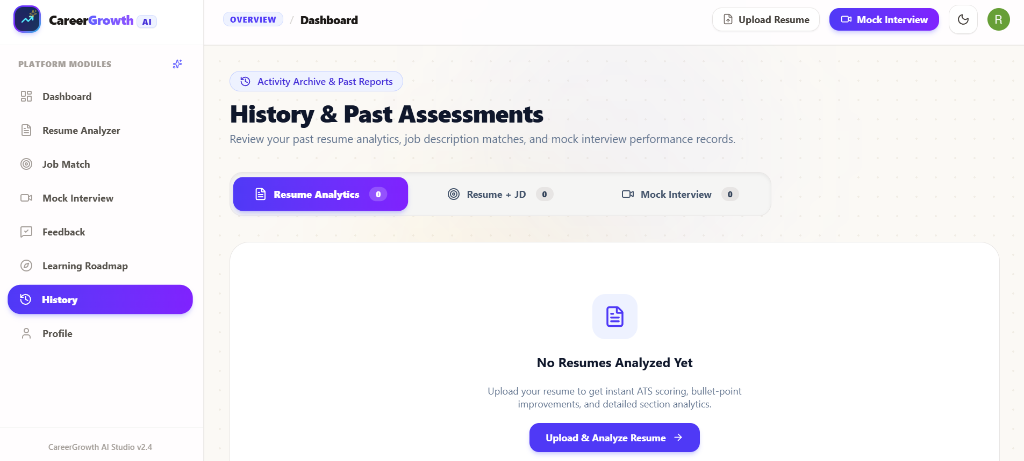
\includegraphics[width=\linewidth]{paper_images/fig5_history_archive.png}
\caption{History and Past Assessments dashboard, archiving resume, job-match, and interview records.}
\label{fig:history}
\end{figure}

Taken together, the latency figures in Table~\ref{tab:metrics} and the persistence guarantees of the history studio support the platform's central design goal: a candidate should be able to run a full diagnostic-and-rehearsal loop---resume score, job match, five-round spoken interview, and consolidated feedback---inside a single sitting, without waiting on a human reviewer or a slow, file-upload-based transcription service.

\section{Conclusions and Future Work}
Resume quality and interview rehearsal are two of the highest-leverage, lowest-access points in the modern hiring process, and \textbf{CareerGrowth AI} targets both from a single, resume-aware diagnostic core rather than treating them as separate tools. By grounding every generated question and every scored answer in the candidate's own verified background, the platform gives feedback that reads as specific and earned rather than generic, and the persisted history studio lets that feedback compound across sessions instead of being lost after each attempt.

Planned future work includes an automated resume-building module that turns a structured intake of a candidate's experience directly into a polished, ATS-ready document, and a real-time facial-expression and vocal-confidence tracking layer during mock interviews---extending the current text-and-speech evaluation with the nonverbal signal that, per the 7-38-55 finding cited in Section~II, plays an outsized role in how an answer actually lands with a human interviewer.

\begin{thebibliography}{00}
\bibitem{b1} J. M. C. J., M. Sabi, M. Benson, G. Baburaj, and S. S., ``Q\&AI: An AI powered mock interview bot for enhancing the performance of aspiring professionals,'' \textit{2024 International Conference on Recent Advances in Electrical, Electronics, Ubiquitous Communication, and Computational Intelligence (RAEEUCCI)}, Chennai, India, 2024, pp. 1--5.
\bibitem{b2} Y. -C. Chou, F. R. Wongso, C. -Y. Chao, and H. -Y. Yu, ``An AI mock-interview platform for interview performance analysis,'' \textit{2022 10th International Conference on Information and Education Technology (ICIET)}, Matsue, Japan, 2022, pp. 37--41.
\bibitem{b3} R. Pandey, D. Chaudhari, S. Bhawani, O. Pawar, and S. Barve, ``Interview Bot with Automatic Question Generation and Answer Evaluation,'' \textit{2023 9th International Conference on Advanced Computing and Communication Systems (ICACCS)}, vol. 1, pp. 1279--1286, IEEE, 2023.
\bibitem{b4} HireVue, ``Frequently asked questions,'' [Online]. Available: \url{https://www.hirevue.com/candidates/faq}
\bibitem{b5} W. Uriawan, R. I. H. Widodo, R. Ramadita, R. F. Herdiyanto, R. S. Marsaputra, and S. Nurrobianti, ``Implementing large language model API for interview training based on job description,'' \textit{Preprints}, Jul. 2024.
\bibitem{b6} D. Harwell, ``A face-scanning algorithm increasingly decides whether you deserve the job,'' \textit{The Washington Post}, Nov. 6, 2019.
\bibitem{b7} A. K. Sinha, M. A. K. Akhtar, and M. Kumar, ``Automated resume parsing and job domain prediction using machine learning,'' \textit{Indian Journal of Science and Technology}, vol. 16, no. 26, pp. 1967--1974, 2023.
\bibitem{b8} MAYO Human Capital, ``Comparison of AI interview systems: Effectively recruit talents with Lasso,'' [Online]. Available: \url{https://www.mayohr.com/tw/blog/detail/Lasso-AI-interview}
\bibitem{b9} R. Venkatesan, S. Shirly, M. Selvarathi, and T. J. Jebaseeli, ``Human emotion detection using DeepFace and artificial intelligence,'' \textit{Engineering Proceedings}, vol. 59, no. 1, p. 37, 2023.
\bibitem{b10} A. Mehrabian and S. R. Ferris, ``Inference of attitudes from nonverbal communication in two channels,'' \textit{Journal of Consulting Psychology}, vol. 31, no. 3, pp. 248--252, 1967.
\bibitem{b11} Y. Adepu, V. R. Boga, and S. U., ``Interviewee performance analyzer using facial emotion recognition and speech fluency recognition,'' \textit{2020 IEEE International Conference for Innovation in Technology (INOCON)}, 2020, pp. 1--5.
\bibitem{b12} L. Chen, R. Zhao, C. W. Leong, B. Lehman, G. Feng, and M. E. Hoque, ``Automated video interview judgment on a large-sized corpus collected online,'' \textit{2017 Seventh International Conference on Affective Computing and Intelligent Interaction (ACII)}, 2017.
\bibitem{b13} I. Naim, M. I. Tanveer, D. Gildea, and M. E. Hoque, ``Automated analysis and prediction of job interview performance,'' \textit{IEEE Transactions on Affective Computing}, vol. 9, no. 2, pp. 191--204, 2018.
\bibitem{b14} R. Mandal, P. Lohar, D. Patil, A. Patil, and S. Wagh, ``AI-Based mock interview evaluator: An emotion and confidence classifier model,'' \textit{2023 International Conference on Intelligent Systems for Communication, IoT and Security (ICISCoIS)}, 2023, pp. 521--526.
\bibitem{b15} Google, ``Interview Warmup - Grow,'' \textit{Grow with Google}, Dec. 2023. [Online]. Available: \url{https://grow.google/certificates/interview-warmup/}
\bibitem{b16} InterviewBot, ``AI-driven interview practice tool,'' [Online]. Available: \url{https://interviewbot.com/}
\bibitem{b17} R. Verrap, E. Nirjhar, A. Nenkova, and T. Chaspari, ``Am I answering my job interview questions right? An NLP approach to predict degree of explanation in job interview responses,'' \textit{Proceedings of the Second Workshop on NLP for Positive Impact (NLP4PI)}, Dec. 2022, pp. 122--129.
\end{thebibliography}

\end{document}
